% questions.tex —— 1977 年·内蒙古卷·文科 · 题目内容片段（无答案）
% 由 tools/generate_projects.py 依来源总账自 1977/1977_数学真题_内蒙古文_试题.md 生成，勿手改（改源 MD 后重跑）


\gkpart{数学试卷（内蒙古文科）}

\begin{gktip}
\textbf{来源说明}：本题面依据固定源 PDF《1977 内蒙古文科数学》印刷页 1 转录。该固定 PDF 是一份题面与解答连续出现的扫描材料：第 1 页给出四道正式题的完整题面，第 1—4 页还载有对应解答。以下题面严格保留第 1(3) 根式中的负号；源解答在计算时将其按正号处理，相关冲突见答案要点与解析正文。正式题量按源材料的题号为 1—4。
\end{gktip}

\begin{question}
\gkti{1}\textbf{（42 分）} 计算或求解下列各题：

（1） 计算 $\sin(-990^\circ)$。

（2） 化简 $\sqrt{4-12a+9a^2}$。

\Needspace{5\baselineskip}
（3） 计算

\nopagebreak[4]
\[
\frac{(-27)^3\sqrt{\left(-\frac{1}{16}\right)^{-\frac12}}}
{(-9)^0\left(\frac32\right)^7\left(\frac12\right)^{-5}}
\]

（4） 已知 $\lg2=0.3010$，$f(x)=\log_{\sqrt{10}}x$，求 $f(5)$。

\Needspace{5\baselineskip}
（5） 求函数

\nopagebreak[4]
\[
y=\frac{\sqrt{1-\frac23x}}{\sqrt[3]{3x-1}}
\]

的定义域。

\Needspace{5\baselineskip}
（6） 已知 $\sin\theta=0.6$，求

\nopagebreak[4]
\[
\left(\sin\frac\theta2-\cos\frac\theta2\right)^2
\]

的值。

\Needspace{0.4\textheight}
\end{question}
\begin{question}
\gkti{2}\textbf{（20 分）} 

（1） 已知：梯形 $ABCD$，$AD\parallel BC$，对角线 $AC$ 和 $BD$ 相交于 $E$，过 $E$ 作平行于底的直线，交 $AB$ 于 $M$，交 $CD$ 于 $N$。求证：$ME=EN$。
\nopagebreak[4]
\begin{center}% 1977 年内蒙古卷文科第 2(1) 题：梯形对角线与平行截线
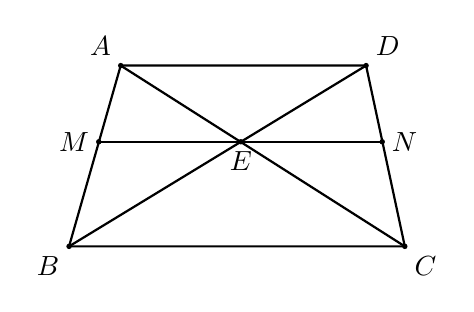
\begin{tikzpicture}[scale=0.82]
  \coordinate (A) at (0.8,2.8);
  \coordinate (D) at (4.6,2.8);
  \coordinate (B) at (0,0);
  \coordinate (C) at (5.2,0);
  \coordinate (E) at (2.66,1.62);
  \coordinate (M) at (0.46,1.62);
  \coordinate (N) at (4.85,1.62);
  \draw[thick] (A)--(D)--(C)--(B)--cycle;
  \draw[thick] (A)--(C);
  \draw[thick] (B)--(D);
  \draw[thick] (M)--(N);
  \fill (A) circle (1.2pt) node[above left] {$A$};
  \fill (D) circle (1.2pt) node[above right] {$D$};
  \fill (B) circle (1.2pt) node[below left] {$B$};
  \fill (C) circle (1.2pt) node[below right] {$C$};
  \fill (E) circle (1.2pt) node[below] {$E$};
  \fill (M) circle (1.2pt) node[left] {$M$};
  \fill (N) circle (1.2pt) node[right] {$N$};
\end{tikzpicture}
\end{center}
\nopagebreak[4]
（2） 圆台上底直径为 $12\ \mathrm{cm}$，下底直径为 $24\ \mathrm{cm}$，高为 $8\ \mathrm{cm}$，求圆台的体积和全面积。（$\pi=3.14$，结果精确到 $0.1\ \mathrm{cm^3}$ 或 $0.1\ \mathrm{cm^2}$。）

\end{question}
\begin{question}
\gkti{3}\textbf{（18 分）} 已知：直线 $3x+y=5$ 及 $2x-3y+4=0$ 交于 $A$ 点。求：

（1） 过 $A$ 点且与 $y$ 轴垂直的直线方程；

（2） 过 $A$ 点且与直线 $2x+y+1=0$ 平行的直线方程；

（3） 过 $A$ 点且与直线 $2x+y+1=0$ 垂直的直线方程。

\end{question}
\begin{question}
\gkti{4}\textbf{（20 分）} 红旗拖拉机厂今年元月份生产出一批甲、乙两种型号的拖拉机，其中生产乙型 16 台。从二月份起，甲型每月增产 10 台，而乙型按每月相同增长率逐月递增，又知二月份甲、乙两型拖拉机产量之比是 $3:2$，三月份甲、乙两型产量之和是 65 台，求乙型拖拉机每月的增长率及甲型拖拉机元月份的产量。

\end{question}